\documentclass{article}[a4paper]
\usepackage{graphicx} % Required for inserting images
\usepackage{tabularx}
\usepackage{geometry}
\usepackage{amsmath}
\usepackage{float} % Add this line to use the 'float' package
\usepackage{siunitx} % Adds ability to use SI units
\usepackage{dirtytalk} % Add Quotations
\usepackage{tabularx}
\usepackage{tikz}
\usetikzlibrary{external}
\tikzexternalize

\title{BEP Vision System}
\author{Z.K.Hahn \\ R. Koopman \\ M. Riedeman \\ S.E. Schimmel}
\date{October 2023}

\begin{document}

\maketitle
\newpage
\section{Introduction}
The TU Delft department of Cognitive Robotics (CoR) has the long term goal of developing robots for logistic applications, which can be extended in the future toward outdoor robots. For our Bachelor Final Project (BEP), we are tasked with the design and creation of a vision system for such a robot.

The required vision system should enable the robot to autonomously navigate and provide metric depth information in order to control a robotic arm for object manipulation. Our project builds on top of the previous BEP group's work, which resulted in the robotic vehicle seen below. Parallel to us another BEP group is working on the creation of the robotic arm that is to be mounted to this very same vehicle.

Since the vision system is intended to be implemented in various robots in the future, keeping the cost of this system to a minimum without compromising performance is crucial. Therefore distance measuring techniques which use LiDAR, structured light 3D scanning or Ultrasonic sensors will not be suitable. Instead one or multiple low-cost camera modules should be used.

\newpage

\section{Project Requirements}
The vision system for this project must adhere to the following requirements:

\begin{enumerate}
    \item \textbf{Source of Input:} The system should exclusively rely on input from camera(s) and not                      incorporate other sensing technologies such as lidar.
    
    \item \textbf{Metric Values:} The vision system is required to provide metric values and not relative                   distances.
    
    \item \textbf{Real-time Depth Data:} The system must be capable of delivering real-time depth data at a         rate of 20 frames per second. This frame rate is chosen based on the robot's top speed which            we assumed 10 km/h.
    
    \item \textbf{Operation Modes:} The vision system should function seamlessly both in motion and in                  standstill.
    
    \item \textbf{Cost Constraint:} The total cost of the cameras used in the system should not exceed             50 euros.

    \item \textbf{Accuracy:} The distances should be as accurate to the mm within 1 meter and beyond 1 meter the accuracy should be at least to the decimeter. 

    \item \textbf{Size:} The computing device should be able to fit in a small robot.
    \item \textbf{Light conditions:} The vision system must work in different daylight lighting conditions.
    \item \textbf{Depth map:} The vision system should be able to measure distance from every object in the view.
    \item \textbf{Required distances to measure:} The vision system should be able to measure distance from 10 cm to 10 meter.
\end{enumerate}

\newpage
\section{Selection Criteria}
The criteria for the vision system design are as follows:

\begin{enumerate}
    \item \textbf{Cost Efficiency:} The entire vision system should be cost-effective, aiming for the lowest    	           possible expenditure without compromising functionality or quality.

    \item \textbf{Energy Efficiency:} The entire vision system should be as energy efficient as possible.

    \item \textbf{Speed:} The refresh-rate of the depth data should be as high as possible.

    \item \textbf{Accuracy:} The displayed distances should be as accurate as possible.

    \item \textbf{Field of View:}  The extent of the observable environment captured by the system should be suitable to the robot's speed. 

    \item \textbf{Compatibility with 'MIRTE' and 'ROS':} Ideally, the system should be compatible with 'MIRTE' (replace 'MIRTE' with the specific software or platform name) and 'ROS' (Robot Operating System), ensuring seamless integration and interoperability with existing technologies.

    \item \textbf{Weight:} The required hardware for the vision system should be as light as possible.

\end{enumerate}

We plan to assign specific weights to each criterion during the evaluation process. These weighted criteria will guide our decision-making, helping us determine the best vision system for our project.

\newpage
\section{Exploring different solutions}

\subsection{Structure from motion (SfM)}
Structure from motion is a technique to obtain a 3D representation from 2D pictures. It relies on that fact that objects further away from the camera move slower than features corresponding to objects closer to the camera. Through analysis of these motion disparities it is possible to construct a 3D structure from 2D images.

This method can work with only one camera but its effectiveness is dependent on motion. If there is no movement, it is not possible to compare different speeds and calculate depth. The camera used for structure from motion needs to be calibrated.

\subsection{Stereo camera vision}
Stereo camera vision uses two cameras with a known distance between them. The further away an object is, the smaller the the displacement of the object between the images from the different cameras. The displacement of pixels in two images corresponding to the same feature, is called the disparity. From this disparity it is possible to calculate the depth. As for structure from motion, this method also requires the cameras to be calibrated.

\subsection{Monocular depth estimation}
Monocular depth estimation uses only one camera. It is able to estimate the depth of every pixel in an image, through a trained neural network. This network is trained on all kinds of data ranging from stereo displacement maps, to LiDAR and sonar data. This makes it possible to estimate depth from a single image.

The training of such models is quite computationally intensive, but inference on a trained model might be feasible on a Raspberry Pi if you use a small model for example. Luckily there are pre-trained models available to download, use and maybe fine-tune.

\subsection{Structured light}
Structured light is a method which uses a camera and a projector which projects a structured pattern on a surface. The camera observes how the pattern is deformed by the shape of the surface. This deformation allows for the derivation of depth information.

This method thus uses a small projector, which can be expensive. If the projector would project the pattern with infrared light then it might not work well if there is a lot of sunlight.

\subsection{Object detection with distance}
Object detection with distance is a way of doing object detection that incorporates distance values. In 'normal' object detection a neural network guesses where objects are in the image. By including depth data in the training process, the network can also estimate how far each detected object is from the camera.

It's also possible to add an inertial measurement unit (IMU) which uses data regarding linear as well as angular accelerations to determine depth.

As for monocular depth estimation, the training of an object detection model (with or without distance) is also computationally intensive. Object detection models that also estimate distance are not as common as monocular depth estimation models and thus more difficult to find.

\subsection{Time-of-Flight Camera}
The Time-of-Flight (ToF) method employs an infrared light source that emits controlled pulses of light, which are subsequently captured by a specialized camera. By precisely measuring the duration between the initial emission and the reception of these light pulses, the ToF system calculates the spatial depth of the objects within its field of view.

\subsection{Depth from (De)focus}
If you have a camera with variable focus, then it is possible to estimate depth without AI models. There are two focus based methods: depth from focus and depth from defocus. Depth from focus compares different pictures with different features in focus. Depth from defocus only takes one picure and estimates the amount of blur and calculates the depth with this amout of blur.

\subsection{Comparison}

The vision system we plan to develop has to be able to work with only one or more cameras. For our requirements, all other sensors are off limits. Therefore only structure from motion, stereo camera vision, monocular depth estimation, object detection with distance remain viable options.

One of the goals of the vision system is to help inform the robot in operating a possible robot arm. This must also work while at rest, so structure from motion is not suitable for our project.

The difference between monocular depth estimation and object detection with distance is that monocular depth estimation tries to guess the depth immediately while object detection with distance tries to detect objects first, before estimating distance. If an object would not be detected, the distance would not be known to the robot and it could crash. Because depth estimation is our main goal, we want to explore monocular depth estimation further instead of the object detection method.
\\
To conclude, we have two viable solutions to our problem: Stereo camera vision and monocular depth estimation. These are the two methods which fit best with the requirements and criteria stated earlier. Hence further research and development will be conducted for these two options.

\newpage
\subsection{Plan for continuation}

After reviewing the possible vision systems with the requirements, only two vision systems remained: monocular depth estimation and stereo camera vision. Our plan is to further investigate these two options in order to assess the performance of each vision system for each criterion. Our performance criterion with the chosen weight are showed in Table \ref{tab:criteria_weights}. 
\\

\begin{table}[H]
    \centering
    \begin{tabular}{|c|c|}
        \hline
        \textbf{Performance criteria} & \textbf{Weight (1-10)} \\
        \hline
        Cost efficiency & 5 \\
        Energy efficiency & 2 \\
        Speed & 2 \\
        Accuracy & 10 \\
        Field of view & 5 \\
        Compatibility with ROS & 2 \\
        Weight & 2 \\
        \hline
    \end{tabular}
    \caption{Weights for Criteria}
    \label{tab:criteria_weights}
\end{table}

First of all, we are going to calculate the required processing power for each system to check whether it can run on a small computing device like a Rasberry Pi. \\
Perhaps some criterion can only be determined with a build vision system. In that case we are planning to build both systems and benchmark the performance of each vision system.https://www.overleaf.com/project/651ab4c6c021ebb58d4f000c

\newpage
\section{Test Results}
\subsection{Monocular Depth Estimation using Deep Learning}

Estimating the depth of a scene from a single image is a task that humans find easy, but it poses significant challenges for computational models aiming for high accuracy while using minimal resources. This task, known as Monocular Depth Estimation (MDE), involves determining depth from a single RGB image. Humans excel in this task due to their ability to utilize various cues such as perspective, scale in relation to known objects, lighting, and occlusion. However, for computational models, MDE is a complex problem because it involves transforming a 3D scene into a 2D projection captured by a camera. This transformation leads to an ill-posed problem where a single 2D image can correspond to an infinite number of different 3D scenes.
\newline

Upon exploring the Monocular Depth Estimation (MDE) using deep learning method, we sought to create a demonstration utilizing a webcam as a camera. Given the open-source nature of many of these models, implementation seemed feasible. The first MDE model we chose testing was MiDaS v2.1 \cite{MiDaS}. Since the MiDaS model is specifically mentioned on the Pytorch website itself and has a large amount of documentation available, we believed this would be a good place to start. Running this model on our laptop, we achieved a sufficient framerate of approximately 32 FPS. However when we tried to run the same model on the NVIDIA Jetson Nano, we encountered several issues:
\begin{enumerate}
    \item There was a hefty latency of approximately 2.5\si{s} between real-time events and the output, although this is most likely not caused by the MiDaS model itself.
    \item The Jetson Nano was only capable of delivering 4 FPS when using MiDaS v2.1, which is far below the requirements.
    \item After further research it became apparent that MiDaS is only able to provide a relative depth map and an additional sensor is required to convert this into a metric depth map.
\end{enumerate}

This led us to search for a version that could provide metric data. Our investigation led us to the ZoeD-M120-N model mentioned in Bhat et al.'s work on ZoeDepth \cite{bhat2023zoedepth}. Titled "ZoeDepth: Zero-shot Transfer by Combining Relative and Metric Depth" \cite{ranking-MDE} the model seemed promising. This model was first of all chosen because it is one of the top performers when tested on the the NYU-Depth V2 dataset \cite{NYU-DepthV2}, which strictly contains indoor scenes. On top of this, there is a lot more community support for troubleshooting, ultimately lead us to prefer this over the VPD \cite{zhao2023unleashing} model, even though it performs a tiny fraction worse in terms of RSME (= root mean square error) when benchmarked on the NYU-Depth V2 dataset. In comparison to MiDaS, the essential advantage of ZoeDepth is the capacity to provide a depth map with metric distance values without the need for an extra sensor. The ability to obtain metric depth data using MDE is crucial because it’s one of our requirements. We wrote a Python script for the ZoeDepth model to use a real-time camera feed instead of single images and ran the model. Sadly ZoeDepth would only run on our laptop, achieving a frame rate of 5 FPS. Trying out the model on the Jetson Nano multiple times, kept resulting in an error message stating the application had been \say{killed} as a result of insufficient memory.
\newline

After this setback we continued our search for a suitable MDE model and came across DistDepth\cite{wu2022toward}. This model has also been specifically trained to tackle unseen complex indoor scenes, unlike many other works which mainly focus on driving scenes and are trained on large-scale driving datasets such as KITTI\cite{geiger2013vision} and Cityscapes\cite{cordts2015cityscapes}. DistDepth not only provides metric depth estimation, it also achieves the RMSE when tested on the NYU-Depth V2 self-supervised and VA (Virtual Apartment) benchmarks \cite{MDE}. Operating the DistDepth model on our laptop we achieved a real-time metric depth map with a frame rate of 22 FPS. Unfortunately the NVIDIA Jetson Nano was unable to replicate this result, since the it completely froze when trying to run DistDepth. Opening the task manager while trying to run the model indicated that, most likely, the DistDepth model wouldn't run at all because of not having enough memory available.

\subsubsection{Conclusion}
To conclude, given our requirements, MDE using deep learning is not a sufficient solution for our computer vision system. The reason is twofold:
Although MDE models which can provide metric depth estimation exists, the NVIDIA Jetson Nano is unable to run such models. The NIVIDA Jetson Nano was only barely able to run the MiDaS model, at a meager frame rate of 4 FPS instead of the desired 20 FPS. Besides not reaching the frame rate target, using the MiDaS model would require an additional sensor to be attached to the system, in order to transform the relative depth map into metric, which wouldn't comply with the requirements. 
Please find below a table summarizing the test results:

\begin{center}
    \begin{table}[H]
    \centering
    \begin{tabular}{|c|c|c|c|} 
        \hline
        \textbf{MDE Deep Learning Model} & \textbf{FPS on Laptop} & \textbf{FPS on NVIDIA Jetson Nano} & \textbf{Metric Depth Map}  \\ 
        \hline
        MiDaS V2.1                                             & 32                                          & 7                                                       & No                                              \\ 
        ZoeDepth                                               & 4                                           & N/A                                                     & Yes                                             \\ 
        DistDepth                                              & 22                                          & N/A                                                     & Yes                                             \\
        \hline
    \end{tabular}
    \caption{Test results of Monocular Depth Estimation using deep learning models}
    \end{table}
\end{center}

\newpage
\subsection{Focus-Based Depth Estimation}

Depth estimation through focus can be accomplished using two main methods: depth from focus and depth from defocus.

\subsubsection{Depth from Focus}

Depth from focus involves creating a focus stack with 10 to 20 photos to determine the depth within a scene. Each photo in the stack is taken at a different focus setting. When we need to find the distance to an object in the scene, we choose the photo where the object is sharpest. By applying Gaussian's lens law, we can then calculate the depth of the object in the scene.

Unfortunately, applying this method in real-time is challenging because it requires capturing 10 to 20 photos for every frame. With our requirement of achieving a frame rate of 20 frames per second (FPS), our vision system would need to process a minimum of 200 photos per second, making it impractical.

Assuming our camera is capable of achieving this framerate, another challenge arises. Each photo in a focus stack requires a distinct focus setting, necessitating rapid adjustments by the camera. For instance, if a frame rate of 20 FPS is desired, the camera must switch focus settings 180 times per second, resulting in a maximum focus-switching time of 1/180 seconds.

One potential solution to address this issue is to use 10 cameras simultaneously. However, this will exceed our budget. In conclusion, Depth from Focus does not meet our real-time processing requirements. Now, let's explore whether Depth from Defocus might offer a more feasible alternative.

\subsubsection{Depth from Defocus}


\newpage
\subsection{Stereo Camera Vision}
\subsubsection{Set Up}
This method consists of two single cameras which are combined to form a stereo set up. Both cameras are connected to the Jetson Nano which posses two camera inputs. To properly gather depth from the stereo set up the cameras first need to be calibrated separately to ensure the most optimal configuration.

\subsubsection{Calibration}
As mentioned earlier, the first step in the calibration process is calibration each camera individually.
\\We followed the same procedure as explained in the Stereo Vision Camera Calibration with OpenCV video \cite{youtube}. This method calibrates each individual camera by taking multiple images of an object of which the dimensions are known, in this case a checkerboard. By rotating, translating and tilting this known object, a camera matrix, distortion parameters, rotation and translation vectors are compute which allows us to remove distortion and results in an un-calibrated Stereo setup.
\\ To create a calibrated setup we use a method called Scale-Invariant Feature Transform (SIFT) 


\subsubsection{Optimization}
To improve the depth map we have tested and analysed different methods. When it comes to stereo vision, there are two main methods that are genereally used; Stereo Block Matching (BM) and Stereo Semi-Global Block Matching (SGBM). 
\\ With StereoBM both images are divided into small blocks and then matched between the left and right image to find the disparities. The idea is that corresponding points in the left and right images will have similar pixel intensities in their respective blocks.
\\ StereoSGBM is an extension to the Block Matching method by also including information from multiple directions (not just the immediate neighbors), which helps in finding more accurate disparities. It takes into account the relationships between pixels across the entire image. 
\\ Research shows that the caption time of a self-captured image 2.083 seconds is for StereoSGBM and 0.814 second for StereoBM \cite{Verma_Verma_2018}. This means that StereoSGBM takes more than 2.5 times to capture the same image. Since the computational power of the Jetson Nano and the Raspberry Pi are limited due to the budget restriction and the desire is to have a real-time vision system, our preference goes to StereoBM as this takes less time to compute. 
\bigskip
\\ Another way to improve the depth map in general is to add a filter to the overall disparity map. One of which is implementing a Weighted Least Error (WLS) filter. By implementation of this filter the noise in the depth map is reduced which enhances the quality of it. This method takes into consideration the error of the disparity measurements and applies weights to different pixel values within the image which results in a more trustworthy disparity values.
\\ The parameters of this method are lamda and sigma. In which lamda determines the level of smoothness of the map. The trade off being that a high smooth surface finish results in a lower distinction between different objects. Sigma is the parameter controlling the chromaticity where a high sigma value equals more attention to colour information where as a lower sigma focus more on geometric information.  
\newpage

\appendix
\section{How does a camera work}
A camera projects a 3D scene to a 2D plane and captures this 2D image.
The camera thus fulfills two functions: projection and capturing. 
We will briefly touch on capturing images, but we are mostly interested in the projection from a 3D scene to a 2D image.

The name camera comes from 'camera obscura', which means dark room. 
The simplest form of a camera is just this: a dark room with a small hole. 
Light travels through this hole and the outside world is projected upside-down on the wall behind the hole.

With modern cameras lenses are added to let in more light and they can capture the light into an image through film or digital sensors, but fundamentally nothing really has changed.
That is why we often use the 'pinhole camera model' to think about cameras.

\subsection{Pinhole Camera Model}

\begin{center}
    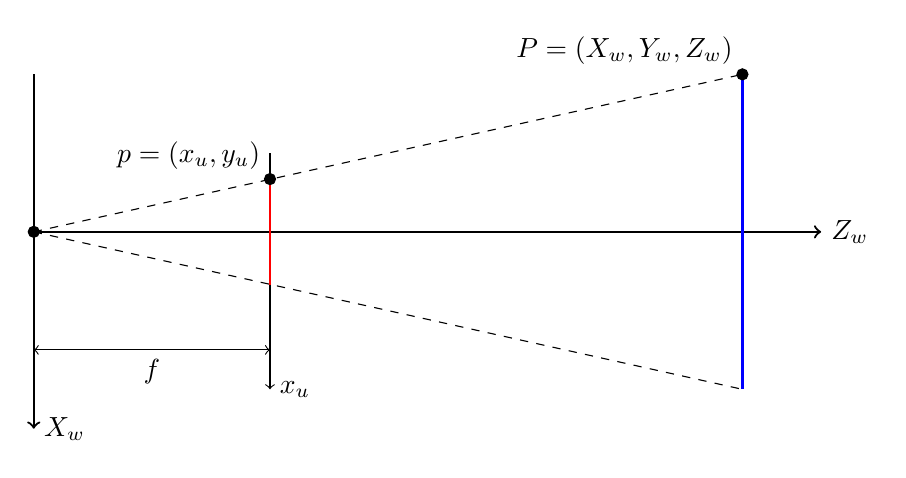
\begin{tikzpicture}
    \draw[thick, ->] (0, 2) -- (0, -2.5) node[anchor=west] {$X_w$};
    \draw[thick, ->] (0, 0) -- (10, 0) node[anchor=west] {$Z_w$};
    \filldraw (0,0) circle (2pt);

    \draw[->] (3, 1) -- (3, -2) node[anchor=west] {$x_u$};

    \draw[<->] (0, -1.5) -- (3, -1.5) node[midway, below] {$f$};

    \draw[red, thick] (3, 0.67) -- (3, -0.67);
    \draw[blue, thick] (9, 2) -- (9, -2);
    
    \draw[thin, dashed] (0, 0) -- (9, 2);
    \draw[thin, dashed] (0, 0) -- (9, -2);

    \filldraw (9, 2) circle (2pt) node[anchor=south east] {$P=(X_w, Y_w, Z_w)$};
    \filldraw (3, 0.67) circle (2pt) node[anchor=south east] {$p=(x_u, y_u)$};

\end{tikzpicture}
\end{center}

The pinhole camera model describes the projection of 3D world coordinates $(X_w, Y_w, Z_w)$ to 2D coordinates on the image plane $(x_u, y_u)$. You can think of a ray of light coming from the world coordinates, traveling through the pinhole and ending up on the image plane. The distance between the image plane and the pinhole, or projection centre, is called the focal length $f$.

In the picture above we've drawn the image plane (in red) before the projection centre to avoid having to think about flipping the image and to keep the diagram compact.

As mentioned earlier the red line in the diagram is the image plane.
To actually capture this image, analog film or a digital sensor is needed. An image sensor converts light waves into small currents that can be read out. 

\subsection{Lenses}
A pinhole is a very small hole. This allows for a crisp picture, but very little light is able to reach the image plane. To be able to control the amount of light entering the camera, we use lenses.

But lenses also complicate the camera. Without a lens, all elements of a scene are in focus. A lens bends the light ...

% TODO -> Watch first principles youtube channel

\subsection{Calibration}
% TODO

\section{OpenCV}

\section{Stereo Matching}

\newpage

\section{Discussion}
\begin{enumerate}
    \item MDE: We hebben niet alle modellen onderzocht.
    \item Future work: Andere sensoren naast de camera's is miss goedkoper
    \item een camera maken die snel genoeg is om focus setting 10 keer in 1/20 van een seconde te veranderen.
\end{enumerate}




\newpage

\bibliography{references}
\bibliographystyle{plain}  % Choose your desired bibliography style
\end{document}


